%------------------------------------------
%	$Id$
%
%	The GMT Documentation Project
%	Copyright (c) 2000-2012.
%	P. Wessel, W. H. F. Smith, R. Scharroo, J. Luis and F. Wobbe
%------------------------------------------
%
\chapter{\gmt\ Map Projections}
\label{ch:6}

\GMT\ implements more than 30 different projections.  They all project the input coordinates
longitude and latitude to positions on a map.  In general, $x' = f(x,y,z)$ and $y' = g(x,y,z)$, where
$z$ is implicitly given as the radial vector length to the $(x,y)$ point on the chosen ellipsoid.  The functions $f$ and $g$ can be
quite nasty and we will refrain from presenting details in this document.  The interested read is referred to
\emph{Snyder} [1987]\footnote{Snyder, J. P., 1987, Map Projections \- A Working Manual, U.S. Geological Survey Prof. Paper 1395.}.
We will mostly be using the \GMTprog{pscoast} command to demonstrate each of the projections.
\GMT\ map projections are grouped into four categories depending on the
nature of the projection.  The groups are

\begin{enumerate}
\item Conic map projections
\item Azimuthal map projections
\item Cylindrical map projections
\item Miscellaneous projections
\end{enumerate}

Because $x$ and $y$ are coupled we can only specify one plot-dimensional scale, typically
a map \emph{scale} (for lower-case map projection code) or a map \emph{width} (for upper-case
map projection code).  However, in some cases it would be more
practical to specify map \emph{height} instead of \emph{width}, while in other situations it would be nice
to set either the \emph{shortest} or \emph{longest} map dimension.  Users may select
these alternatives by appending a character code to their map dimension.  To specify map \emph{height},
append \textbf{h} to the given dimension; to select the minimum map dimension, append \textbf{-}, whereas you may
append \textbf{+} to select the maximum map dimension.  Without the modifier the map width is
selected by default.

In \GMT\ version 4.3.0 we noticed we ran out of the alphabet for 1-letter (and sometimes 2-letter) projection codes. To allow more flexibility, and to make it easier to remember the codes, we implemented the option to use the abbreviations used by the \progname{Proj4} mapping package. Since some of the \GMT\ projections are not in \progname{Proj4}, we invented some of our own as well. For a full list of both the old 1- and 2-letter codes, as well as the \progname{Proj4}-equivalents see the quick reference cards in Section~\ref{sec:purpose}. For example, \Opt{JM15c} and \Opt{JMerc/15c} have the same meaning.

\section{Conic projections}
\index{Projection!conic|(}
\index{Conic projections|(}

\subsection{Albers conic equal-area projection (\Opt{Jb} \Opt{JB})}
\index{Projection!conic!Albers \Opt{Jb} \Opt{JB}|(}
\index{Albers conic projection \Opt{Jb} \Opt{JB}|(}
\index{\Opt{Jb} \Opt{JB} (Albers)|(}

This projection, developed by Albers in 1805, is predominantly
used to map regions of large east-west extent, in particular
the United States.  It is a conic, equal-area projection, in
which parallels are unequally spaced arcs of concentric circles,
more closely spaced at the north and south edges of the map.
Meridians, on the other hand, are equally spaced radii about
a common center, and cut the parallels at right angles.
Distortion in scale and shape vanishes along the two standard
parallels.  Between them, the scale along parallels is too small;
beyond them it is too large.  The opposite is true for the scale
along meridians.  To define the projection in \GMT\ you need to
provide the following information:

\begin{itemize}
\item Longitude and latitude of the projection center.
\item Two standard parallels.
\item Map scale in inch/degree or 1:xxxxx notation (\Opt{Jb}), or map width (\Opt{JB}).
\end{itemize}

Note that you must include the ``1:'' if you choose to specify the
scale that way.  E.g., you can say 0.5 which means 0.5 inch/degree
or 1:200000 which means 1 inch on the map equals 200,000 inches
along the standard parallels.  The projection center defines the
origin of the rectangular map coordinates.  As an example we will
make a map of the region near Taiwan.  We choose the center of
the projection to be at 125 \DS E/20 \DS N and 25 \DS N
and 45 \DS N as our two standard parallels.  We desire a map
that is 5 inches wide.  The complete command needed to generate
the map below is therefore given by: 

\script{GMT_albers} 

\GMTfig[h]{GMT_albers}{Albers equal-area conic map projection}

\index{Projection!conic!Albers \Opt{Jb} \Opt{JB}|)}
\index{Albers conic projection \Opt{Jb} \Opt{JB}|)}
\index{\Opt{Jb} \Opt{JB} (Albers)|)}

\subsection{Equidistant conic projection (\Opt{Jd} \Opt{JD})}
\index{Projection!conic!Equidistant \Opt{Jd} \Opt{JD}|(}
\index{Equidistant conic projection \Opt{Jd} \Opt{JD}|(}
\index{\Opt{Jd} \Opt{JD} (Equidistant conic)|(}

The equidistant conic projection was described by the Greek
philosopher Claudius Ptolemy about A.D.\ 150.  It is neither
conformal or equal-area, but serves as a compromise between them.
The scale is true along all meridians and the standard parallels.
To select this projection in \GMT\ you must
provide the same information as for the other conic projection, i.e.,

\begin{itemize}
\item Longitude and latitude of the projection center.
\item Two standard parallels.
\item Map scale in inch/degree or 1:xxxxx notation (\Opt{Jd}), or map width (\Opt{JD}).
\end{itemize}

The equidistant conic projection is often used for atlases with
maps of small countries.  As an example, we generate a map of
Cuba:

\script{GMT_equidistant_conic} 

\GMTfig[h]{GMT_equidistant_conic}{Equidistant conic map projection}

\index{Projection!conic!Equidistant \Opt{Jd} \Opt{JD}|)}
\index{Equidistant conic projection \Opt{Jd} \Opt{JD}|)}
\index{\Opt{Jd} \Opt{JD} (Equidistant conic)|)}

\subsection{Lambert conic conformal projection (\Opt{Jl} \Opt{JL})}
\index{Projection!conic!Lambert \Opt{Jl} \Opt{JL}|(}
\index{Lambert conic projection \Opt{Jl} \Opt{JL}|(}
\index{\Opt{Jl} \Opt{JL} (Lambert conic)|(}

This conic projection was designed by the Alsatian mathematician Johann Heinrich Lambert (1772) and has been
used extensively for mapping of regions with predominantly east-west
orientation, just like the Albers projection.  Unlike the Albers
projection, Lambert's conformal projection is not equal-area.
The parallels are arcs of circles with a common origin, and
meridians are the equally spaced radii of these circles.  As with
Albers projection, it is only the two standard parallels that are
distortion-free.  To select this projection in \GMT\ you must
provide the same information as for the Albers projection, i.e.,

\begin{itemize}
\item Longitude and latitude of the projection center.
\item Two standard parallels.
\item Map scale in inch/degree or 1:xxxxx notation (\Opt{Jl}), or map width (\Opt{JL}).
\end{itemize}

The Lambert conformal projection has been used for basemaps for all
the 48 contiguous States with the two fixed standard parallels
33\DS N and 45\DS N.  We will generate a map of the continental
USA using these parameters.  Note that with all the projections you
have the option of selecting a rectangular border rather than one
defined by meridians and parallels.  Here, we choose the regular WESN
region, a ``fancy'' basemap frame, and use degrees west for longitudes.
The generating commands used were

\script{GMT_lambert_conic} 

\GMTfig[h]{GMT_lambert_conic}{Lambert conformal conic map projection}

The choice for projection center does not affect the projection but
it indicates which meridian (here 100\DS W) will be vertical on
the map.  The standard parallels were originally selected by Adams
to provide a maximum scale error between latitudes 30.5\DS N and
47.5\DS N of 0.5--1\%.  Some areas, like Florida, experience scale
errors of up to 2.5\%.
\index{Projection!conic!Lambert \Opt{Jl} \Opt{JL}|)}
\index{Lambert conic projection \Opt{Jl} \Opt{JL}|)}
\index{\Opt{Jl} \Opt{JL} (Lambert conic)|)}

\subsection{(American) polyconic projection (\Opt{Jpoly} \Opt{JPoly}}
\index{Projection!conic!polyconic \Opt{Jpoly} \Opt{JPoly}|(}
\index{Polyconic projection \Opt{Jpoly} \Opt{JPoly}|(}
\index{\Opt{Jpoly} \Opt{JPoly} (Polyconic)|(}

The polyconic projection, in Europe usually referred to as the American polyconic projection, was introduced shortly before 1820 by the Swiss-American cartographer Ferdinand Rodulph Hassler (1770-1843). As head of the Survey of the Coast, he was looking for a projection that would give the least distortion for mapping the coast of the United States. The projection acquired its name from the construction of each parallel, which is achieved by projecting the parallel onto the cone while it is rolled around the globe, along the central meridian, tangent to that parallel. As a consequence, the projection involves many cones rather than a single one used in regular conic projections.

The polyconic projection is neither equal-area, nor conformal. It is true to scale without distortion along the central meridian. Each parallel is true to scale as well, but the meridians are not as they get further away from the central meridian. As a consequence, no parallel is standard because conformity is lost with the lengthening of the meridians.

Below we reproduce the illustration by \emph{Snyder} [1987], with a gridline every 10\DS{} and annotations only every 30\DS{} in longitude:

\script{GMT_polyconic} 

\GMTfig[h]{GMT_polyconic}{(American) polyconic projection}

\index{Projection!conic!polyconic \Opt{Jpoly} \Opt{JPoly}|)}
\index{Polyconic projection \Opt{Jpoly} \Opt{JPoly}|)}
\index{\Opt{Jpoly} \Opt{JPoly} (Polyconic)|)}

\index{Projection!conic|)}
\index{Conic projections|)}

\clearpage
\section{Azimuthal projections}
\index{Azimuthal projections|(}
\index{Projection!azimuthal|(}

\subsection{Lambert Azimuthal Equal-Area (\Opt{Ja} \Opt{JA})}
\index{Projection!azimuthal!Lambert \Opt{Ja} \Opt{JA}|(}
\index{Lambert azimuthal projection \Opt{Ja} \Opt{JA}|(}
\index{\Opt{Ja} \Opt{JA} (Lambert azimuthal)|(}

This projection was developed by Lambert in 1772 and is
typically used for mapping large regions like continents
and hemispheres.  It is an azimuthal, equal-area projection,
but is not perspective.  Distortion is zero at the center
of the projection, and increases radially away from this
point.  To define this projection in \GMT\ you must provide
the following information:

\begin{itemize}
\item Longitude and latitude of the projection center.
\item Optionally, the horizon, i.e., the number of degrees from the center to the edge ($\le$180\DS, default is 90\DS).
\item Scale as 1:xxxxx or as radius/latitude where radius
is the projected distance on the map from projection center to an oblique
latitude (\Opt{Ja}), or map width (\Opt{JA}).
\end{itemize}

Two different types of maps can be made with this projection
depending on how the region is specified.  We will give
examples of both types.

\subsubsection{Rectangular map}

\index{Region!rectangular}
\index{Region!geographical}

In this mode we define our region by specifying the
longitude/latitude of the lower left and upper right corners
instead of the usual \emph{west, east, south, north} boundaries.
The reason for specifying our area this way is that for this
and many other projections, lines of equal longitude and
latitude are not straight lines and are thus poor choices for
map boundaries.  Instead we require that the map boundaries be
rectangular by defining the corners of a rectangular map boundary.
Using 0\DS E/40\DS S (lower left) and 60\DS E/10\DS S
(upper right) as our corners we try\par 

\script{GMT_lambert_az_rect} 

\GMTfig[h]{GMT_lambert_az_rect}{Rectangular map using the Lambert
azimuthal equal-area projection.}

Note that an ``r'' is appended to the \Opt{R} option to inform
\GMT\ that the region has been selected using the rectangle
technique, otherwise it would try to decode the values as
\emph{west, east, south, north} and report an error since
\emph{'east'} $<$ \emph{'west'}.

\subsubsection{Hemisphere map}
\index{Hemisphere map}

\label{sec:lamb}
Here, you must specify the world as your region (\Opt{Rg} or \Opt{Rd}).
E.g., to obtain a hemisphere view that shows the Americas, try 

\script{GMT_lambert_az_hemi}
\GMTfig[h]{GMT_lambert_az_hemi}{Hemisphere map using the Lambert
azimuthal equal-area projection.}

To geologists, the Lambert azimuthal equal-area projection (with
origin at 0\DS /0\DS ) is known as the \emph{equal-area}
(Schmidt) stereonet and used for plotting fold axes, fault planes,
and the like.  An \emph{equal-angle} (Wulff) stereonet can
be obtained by using the stereographic projection (discussed later).
The stereonets produced by these two projections appear below.\par 

\GMTfig[h]{GMT_stereonets}{Equal-Area (Schmidt) and Equal-Angle (Wulff) stereo nets.}
\index{Stereonet!Schmidt equal-area}
\index{Stereonet!Wulff equal-angle}

\index{Projection!azimuthal!Lambert \Opt{Ja} \Opt{JA}|)}
\index{Lambert azimuthal projection \Opt{Ja} \Opt{JA}|)}
\index{\Opt{Ja} \Opt{JA} (Lambert azimuthal)|)}

\subsection{Stereographic Equal-Angle projection (\Opt{Js} \Opt{JS})}
\index{Projection!azimuthal!stereographic \Opt{Js} \Opt{JS}|(}
\index{Stereographic projection \Opt{Js} \Opt{JS}|(}
\index{\Opt{Js} \Opt{JS} (Stereographic)|(}

This is a conformal, azimuthal projection that dates back to the
Greeks.  Its main use is for mapping the polar regions.  In
the polar aspect all meridians are straight lines and parallels
are arcs of circles.  While this is the most common use it is
possible to select any point as the center of projection.  The
requirements are

\begin{itemize}
\item Longitude and latitude of the projection center.
\item Optionally, the horizon, i.e., the number of degrees from the center to the edge ($<$180\DS, default is 90\DS).
\item Scale as 1:xxxxx (true scale at pole), slat/1:xxxxx
(true scale at standard parallel slat), or radius/latitude where
radius is distance on map in inches from projection center to
a particular [possibly oblique] latitude (\Opt{Js}), or simply map
width (\Opt{JS}).
\end{itemize}

A default map scale factor of 0.9996 will be applied by default
(although you may change this with \textbf{PROJ\_SCALE\_FACTOR}).
However, the setting is ignored when a standard
parallel has been specified since the scale is then implicitly given.
We will look at two different types of maps.

\subsubsection{Polar Stereographic Map} 
\index{Projection!azimuthal!polar}

In our first example we will let the projection center be at
the north pole.  This means we have a polar stereographic
projection and the map boundaries will coincide with lines
of constant longitude and latitude.  An example is given by

\script{GMT_stereographic_polar}
\GMTfig[h]{GMT_stereographic_polar}{Polar
stereographic conformal projection.}

\subsubsection{Rectangular stereographic map} 
\index{Projection!stereographic!rectangular}

As with Lambert's azimuthal equal-area projection we have
the option to use rectangular boundaries rather than the
wedge-shape typically associated with polar projections.
This choice is defined by selecting two points as corners
in the rectangle and appending an ``r'' to the \Opt{R} option.
This command produces a map as presented in
Figure~\ref{fig:GMT_stereographic_rect}:

\script{GMT_stereographic_rect}
\GMTfig[h]{GMT_stereographic_rect}{Polar
stereographic conformal projection with rectangular borders.}

\subsubsection{General stereographic map}
\index{Projection!stereographic!general}

In terms of usage this projection is identical to the Lambert
azimuthal equal-area projection.  Thus, one can make both
rectangular and hemispheric maps.  Our example shows Australia
using a projection pole at 130E/30\DS S.  The command used was

\script{GMT_stereographic_general}

\GMTfig[H]{GMT_stereographic_general}{General
stereographic conformal projection with rectangular borders.}

By choosing 0\DS/0\DS  as the pole, we obtain the conformal
stereonet presented next to its equal-area cousin in the Section~\ref{sec:lamb} on
the Lambert azimuthal equal-area projection (Figure~\ref{fig:GMT_stereonets}).

\index{Projection!azimuthal!stereographic \Opt{Js} \Opt{JS}|)}
\index{Stereographic projection \Opt{Js} \Opt{JS}|)}
\index{\Opt{Js} \Opt{JS} (Stereographic)|)}

\subsection{Perspective projection (\Opt{Jg} \Opt{JG})}
\index{Projection!azimuthal!perspective \Opt{Jg} \Opt{JG}|(}
\index{Perspective projection \Opt{Jg} \Opt{JG}|(}
\index{\Opt{Jg} \Opt{JG} (Perspective)|(}

The perspective projection imitates in 2 dimensions the 3-dimensional view of the
earth from space. The implementation in \GMT\ is very flexible, and thus requires
many input variables. Those are listed and explained below, with the values used in
Figure~\ref{fig:GMT_perspective} between brackets.

\begin{itemize}
\item Longitude and latitude of the projection center (4\DS E/52\DS N).
\item Altitude of the viewer above sea level in kilometers (230 km). If this value is less than
10, it is assumed to be the distance of the viewer from the center of the earth in earth radii.
If an ``r'' is appended, it is the distance from the center of the earth in kilometers.
\item Azimuth in degrees (90\DS, due east). This is the direction in which you are looking, measured
clockwise from north.
\item Tilt in degrees (60\DS). This is the viewing angle relative to zenith. So a tilt of 0\DS\ is
looking straight down, 60\DS\ is looking from 30\DS\ above the horizon.
\item Twist in degrees (180\DS). This is the boresight rotation (clockwise) of the image. The twist
of 180\DS\ in the example mimics the fact that the Space Shuttle flies upside down.
\item Width and height of the viewpoint in degrees (60\DS). This number depends on whether you are
looking with the naked eye (in which case you view is about 60\DS\ wide), or with binoculars, for
example.
\item Scale as 1:xxxxx or as radius/latitude where
radius is distance on map in inches from projection center to
a particular [possibly oblique] latitude (\Opt{Jg}), or map
width (\Opt{JG}) (5 inches).
\end{itemize}

The imagined view of northwest Europe from a Space Shuttle at 230 km looking due east is thus
accomplished by the following \GMTprog{pscoast} command:

\script{GMT_perspective} 

\GMTfig[h]{GMT_perspective}{View from the Space Shuttle in Perspective projection.}

\index{Projection!azimuthal!perspective \Opt{Jg} \Opt{JG}|)}
\index{Perspective projection \Opt{Jg} \Opt{JG}|)}
\index{\Opt{Jg} \Opt{JG} (Perspective)|)}

\subsection{Orthographic projection (\Opt{Jg} \Opt{JG})}

\index{Projection!azimuthal!orthographic \Opt{Jg} \Opt{JG}|(}
\index{Orthographic projection \Opt{Jg} \Opt{JG}|(}
\index{\Opt{Jg} \Opt{JG} (Orthographic)|(}

The orthographic azimuthal projection is a perspective projection
from infinite distance.  It is therefore often used to give the
appearance of a globe viewed from outer space.  As with Lambert's
equal-area and the stereographic projection, only one hemisphere
can be viewed at any time.  The projection is neither equal-area
nor conformal, and much distortion is introduced near the edge
of the hemisphere.  The directions from the center of projection
are true.  The projection was known to the Egyptians and Greeks
more than 2,000 years ago.  Because it is mainly used for
pictorial views at a small scale, only the spherical form is necessary.

To specify the orthographic projection the same options \Opt{Jg} or \Opt{JG} as the perspective
projection are used, but with fewer variables to supply:

\begin{itemize}
\item Longitude and latitude of the projection center.
\item Optionally, the horizon, i.e., the number of degrees from the center to the edge ($\le$90\DS, default is 90\DS).
\item Scale as 1:xxxxx or as radius/latitude where
radius is distance on map in inches from projection center to
a particular [possibly oblique] latitude (\Opt{Jg}), or map
width (\Opt{JG}).
\end{itemize}

Our example of a perspective view centered on 75\DS W/40\DS N
can therefore be generated by the following \GMTprog{pscoast} command: 

\script{GMT_orthographic} 

\GMTfig[h]{GMT_orthographic}{Hemisphere map using the Orthographic projection.}

\index{Projection!azimuthal!orthographic \Opt{Jg} \Opt{JG}|)}
\index{Orthographic projection \Opt{Jg} \Opt{JG}|)}
\index{\Opt{Jg} \Opt{JG} (Orthographic)|)}

\subsection {Azimuthal Equidistant projection (\Opt{Je} \Opt{JE})}

\index{Projection!azimuthal!equidistant \Opt{Je} \Opt{JE}|(}
\index{Azimuthal equidistant projection \Opt{Je} \Opt{JE}|(}
\index{\Opt{Je} \Opt{JE} (Azimuthal equidistant)|(}

The most noticeable feature of this azimuthal projection is the
fact that distances measured from the center are true.  Therefore,
a circle about the projection center defines the locus of points
that are equally far away from the plot origin.  Furthermore,
directions from the center are also true.  The projection, in
the polar aspect, is at least several centuries old.  It is a
useful projection for a global view of locations at various or
identical distance from a given point (the map center).

To specify the azimuthal equidistant projection you must supply:

\begin{itemize}
\item Longitude and latitude of the projection center.
\item Optionally, the horizon, i.e., the number of degrees from the center to the edge ($\le$180\DS, default is 180\DS).
\item Scale as 1:xxxxx or as radius/latitude where
radius is distance on map in inches from projection center to
a particular [possibly oblique] latitude (\Opt{Je}), or map
width (\Opt{JE}).
\end{itemize}

Our example of a global view centered on 100\DS W/40\DS N
can therefore be generated by the following \GMTprog{pscoast}
command.  Note that the antipodal point is 180\DS\ away from
the center, but in this projection this point plots as the
entire map perimeter:

\script{GMT_az_equidistant} 

\GMTfig[h]{GMT_az_equidistant}{World map using the equidistant azimuthal projection.}

\index{Projection!azimuthal!equidistant \Opt{Je} \Opt{JE}|)}
\index{Azimuthal equidistant projection \Opt{Je} \Opt{JE}|)}
\index{\Opt{Je} \Opt{JE} (Azimuthal equidistant)|)}

\subsection{Gnomonic projection (\Opt{Jf} \Opt{JF})}

\index{Projection!azimuthal!gnomonic \Opt{Jf} \Opt{JF}|(}
\index{Gnomonic projection \Opt{Jf} \Opt{JF}|(}
\index{\Opt{Jf} \Opt{JF} (Gnomonic)|(}

The Gnomonic azimuthal projection is a perspective projection
from the center onto a plane tangent to the surface.  Its origin
goes back to the old Greeks who used it for star maps almost 2500
years ago.  The projection is neither equal-area nor conformal,
and much distortion is introduced near the edge of the hemisphere;
in fact, less than a hemisphere may be shown around a given center.
The directions from the center of projection are true.  Great circles
project onto straight lines. Because it is mainly used for pictorial
views at a small scale, only the spherical form is necessary.

To specify the Gnomonic projection you must supply:

\begin{itemize}
\item Longitude and latitude of the projection center.
\item Optionally, the horizon, i.e., the number of degrees from the center to the edge ($<$90\DS, default is 60\DS).
\item Scale as 1:xxxxx or as radius/latitude where
radius is distance on map in inches from projection center to
a particular [possibly oblique] latitude (\Opt{Jf}), or map
width (\Opt{JF}).
\end{itemize}

Using a horizon of 60\DS , our example of this projection
centered on 120\DS W/35\DS N can therefore be generated by
the following \GMTprog{pscoast} command:

\script{GMT_gnomonic} 

\GMTfig[h]{GMT_gnomonic}{Gnomonic azimuthal projection.}

\index{Projection!azimuthal!gnomonic \Opt{Jf} \Opt{JF}|)}
\index{Gnomonic projection \Opt{Jf} \Opt{JF}|)}
\index{\Opt{Jf} \Opt{JF} (Gnomonic)|)}

\index{Azimuthal projections|)}
\index{Projection!azimuthal|)}

\clearpage
\section{Cylindrical projections}
\index{Cylindrical projections|(}
\index{Projection!cylindrical|(}

Cylindrical projections are easily recognized for its shape: maps are rectangular and meridians and parallels are straight lines crossing at right angles. But that is where similarities between the cylindrical projections supported by \GMT\ (Mercator, transverse Mercator, universal transverse Mercator, oblique Mercator, Cassini, cylindrical equidistant, cylindrical equal-area, Miller, and cylindrical stereographic projections) stops. Each have a different way of spacing the meridians and parallels to obtain certain desirable cartographic properties.

\subsection{Mercator projection (\Opt{Jm} \Opt{JM})}
\index{Projection!cylindrical!Mercator \Opt{Jm} \Opt{JM}|(}
\index{Mercator projection \Opt{Jm} \Opt{JM}|(}
\index{\Opt{Jm} \Opt{JM} (Mercator)|(}

Probably the most famous of the various map projections,
the Mercator projection takes its name from the Flemish cartographer Gheert Cremer, better known as Gerardus Mercator, who presented it in 1569.  
The projection is a cylindrical and conformal, with no distortion along the equator.  A major
navigational feature of the projection is that a line of
constant azimuth is straight.  Such a line is called a
rhumb line or \emph{loxodrome}\index{Loxodrome}.  Thus, to sail from one
point to another one only had to connect the points with
a straight line, determine the azimuth of the line, and
keep this constant course for the entire voyage\footnote{This
is, however, not the shortest distance.  It is given
by the great circle connecting the two points.}\index{Great circle}.  The
Mercator projection has been used extensively for world
maps in which the distortion towards the polar regions
grows rather large, thus incorrectly giving the impression
that, for example, Greenland is larger than South America.
In reality, the latter is about eight times the size of
Greenland.  Also, the Former Soviet Union looks much bigger
than Africa or South America.  One may wonder whether this
illusion has had any influence on U.S.\ foreign policy.

In the regular Mercator projection, the cylinder touches
the globe along the equator.  Other orientations like
vertical and oblique give rise to the Transverse and
Oblique Mercator projections, respectively.  We will
discuss these generalizations following the regular
Mercator projection.

The regular Mercator projection requires a minimum of
parameters.  To use it in \GMT\ programs you supply this
information (the first two items are optional and have defaults):

\begin{itemize} 
\item Central meridian [Middle of your map].
\item Standard parallel for true scale [Equator]. When supplied, central meridian must be supplied as well.
\item Scale along the equator in inch/degree or
1:xxxxx (\Opt{Jm}), or map width (\Opt{JM}).
\end{itemize} 

Our example presents a world map at a scale of 0.012
inch pr degree which will give a map 4.32 inch wide.
It was created with the command:

\script{GMT_mercator}

\GMTfig[H]{GMT_mercator}{Simple Mercator map.}

While this example is centered on the Dateline, one can
easily choose another configuration with the \Opt{R} option.
A map centered on Greenwich would specify the region with
\textbf{-R}-180/180/-70/70. 

\index{Projection!cylindrical!Mercator \Opt{Jm} \Opt{JM}|)}
\index{Mercator projection \Opt{Jm} \Opt{JM}|)}
\index{\Opt{Jm} \Opt{JM} (Mercator)|)}

\subsection{Transverse Mercator projection (\Opt{Jt} \Opt{JT})} 
\index{Projection!cylindrical!transverse Mercator \Opt{Jt} \Opt{JT}|(}
\index{Transverse Mercator projection \Opt{Jt} \Opt{JT}|(}
\index{\Opt{Jt} \Opt{JT} (Transverse Mercator)|(}

The transverse Mercator was invented by Lambert in 1772.
In this projection the cylinder touches a meridian along
which there is no distortion.  The distortion increases away
from the central meridian and goes to infinity at 90\DS\ from
center.  The central meridian, each meridian 90\DS\ away
from the center, and equator are straight lines; other parallels
and meridians are complex curves.  The projection is defined
by specifying:

\begin{itemize} 
\item The central meridian.
\item Optionally, the latitude of origin (default is the equator).
\item Scale along the equator in inch/degree or 1:xxxxx (\Opt{Jt}), or map width (\Opt{JT}).
\end{itemize} 

The optional latitude of origin defaults to Equator if not specified.
Although defaulting to 1, you can change the map scale factor via
the \textbf{PROJ\_SCALE\_FACTOR} parameter.
Our example shows a transverse Mercator map of south-east
Europe and the Middle East with 35\DS E as the central
meridian:

\script{GMT_transverse_merc}

\GMTfig[H]{GMT_transverse_merc}{Rectangular Transverse Mercator map.}
 
The transverse Mercator can also be used to generate a global map---the
equivalent of the 360\DS\ Mercator map.  Using the command

\script{GMT_TM}

\noindent
we made the map illustrated in Figure~\ref{fig:GMT_TM}.  Note that
when a world map is given (indicated by \Opt{R}\emph{0/360/s/n}), the arguments
are interpreted to mean oblique degrees, i.e., the 360\DS\ range is
understood to mean the extent of the plot along the central meridian,
while the ``south'' and ``north'' values represent how far from the
central longitude we want the plot to extend.  These values correspond
to latitudes in the regular Mercator projection and must therefore be
less than 90\DS.

\GMTfig[H]{GMT_TM}{A global transverse Mercator map.}

\index{Projection!cylindrical!transverse Mercator \Opt{Jt} \Opt{JT}|)}
\index{Transverse Mercator projection \Opt{Jt} \Opt{JT}|)}
\index{\Opt{Jt} \Opt{JT} (Transverse Mercator)|)}

\subsection{Universal Transverse Mercator (UTM) projection (\Opt{Ju} \Opt{JU})} 
\index{Projection!cylindrical!UTM \Opt{Ju} \Opt{JU}|(}
\index{UTM projection \Opt{Ju} \Opt{JU}|(}
\index{\Opt{Ju} \Opt{JU} (UTM)|(}

A particular subset of the transverse Mercator is the
Universal Transverse Mercator (UTM) which was adopted
by the US Army for large-scale military maps.  Here, the
globe is divided into 60 zones between 84\DS S and
84\DS N, most of which are 6\DS\ wide.  Each of
these UTM zones have their unique central meridian.
Furthermore, each zone is divided into latitude bands
but these are not needed to specify the projection for
most cases.  See Figure~\ref{fig:GMT_utm_zones} for all
zone designations.

\begin{figure}[htb]
   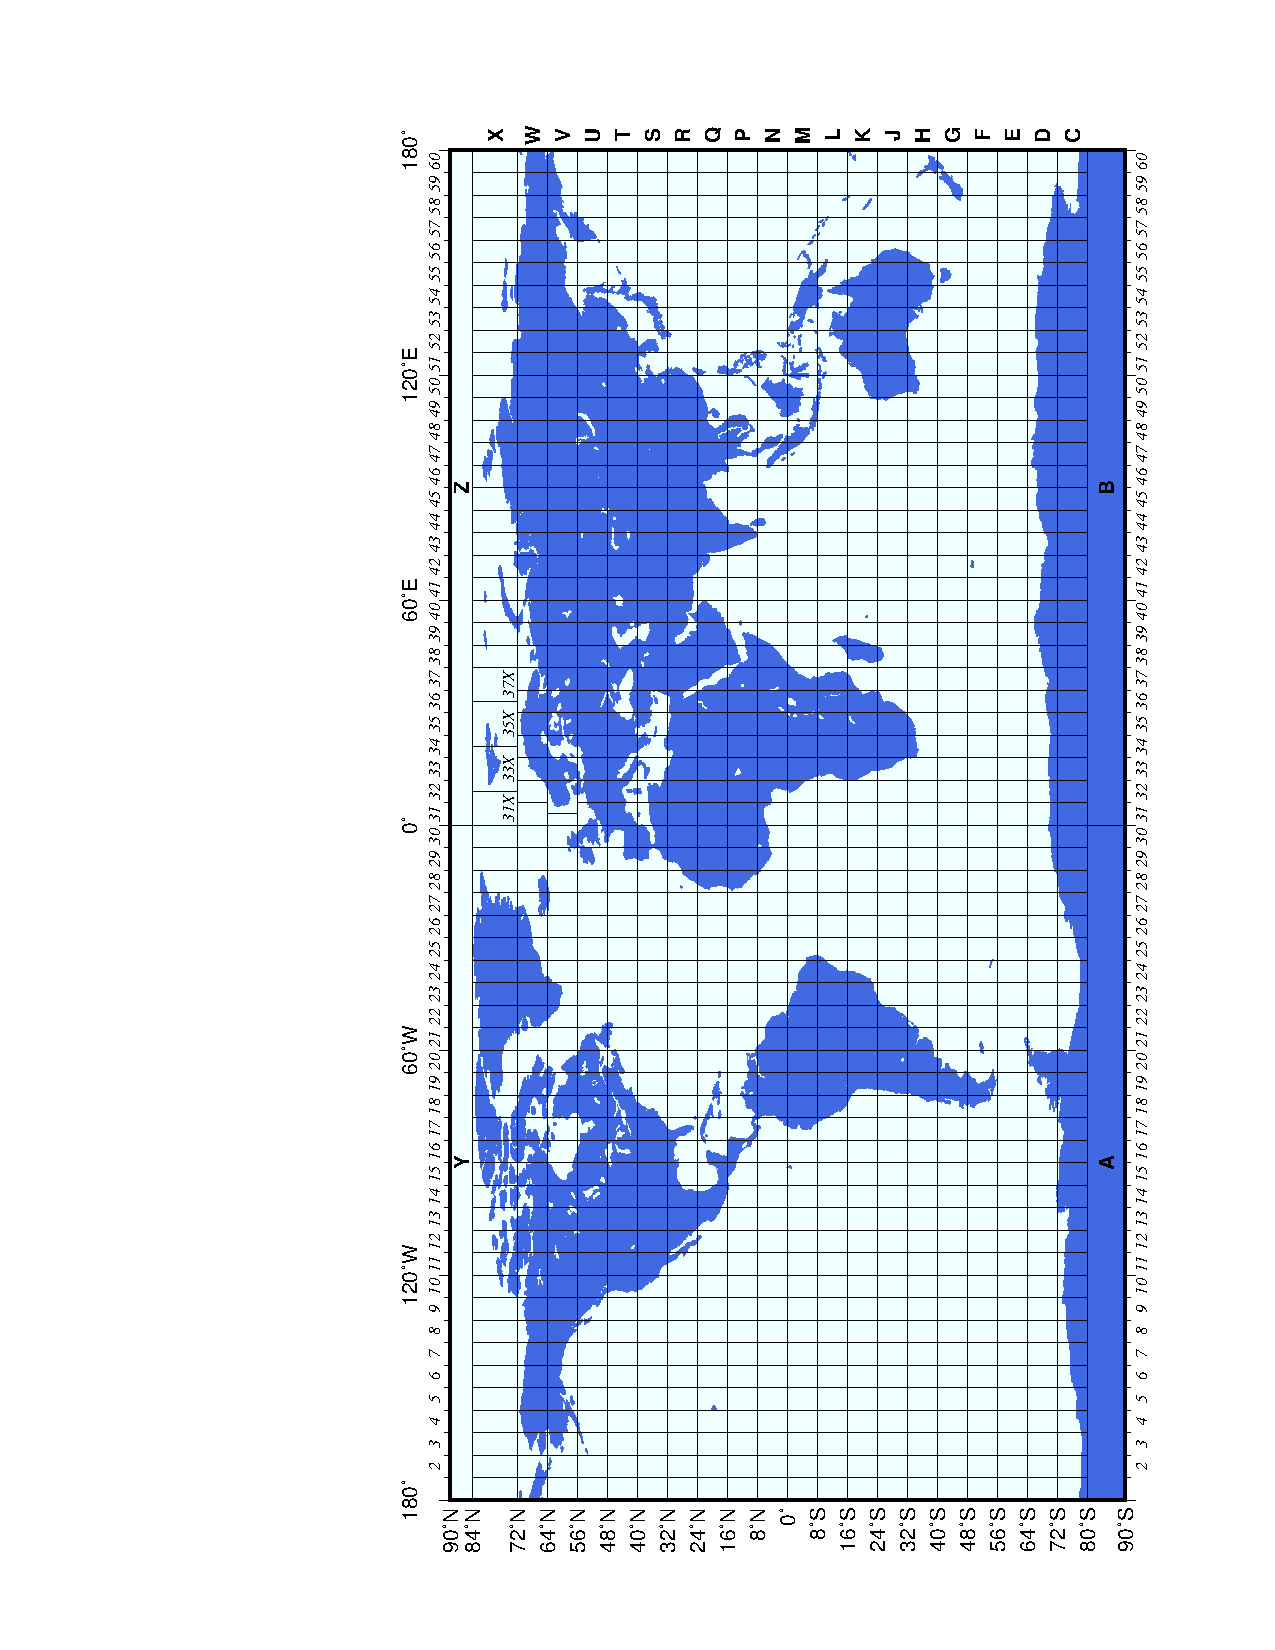
\includegraphics[width=\textwidth]{GMT_utm_zones}
   \caption{Universal Transverse Mercator zone layout.}
   \label{fig:GMT_utm_zones}
\end{figure}

\GMT\ implements both the transverse Mercator and the
UTM projection.  When selecting UTM you must specify:

\begin{itemize} 
\item UTM zone (A, B, 1--60, Y, Z).  Use negative values for numerical zones in the southern hemisphere
or append the latitude modifiers C--H, J--N, P--X) to specify an exact UTM grid zone.
\item Scale along the equator in inch/degree or 1:xxxxx (\Opt{Ju}), or map width (\Opt{JU}).
\end{itemize} 

In order to minimize the distortion in any given zone,
a scale factor of 0.9996 has been factored into the formulae.
(although a standard, you can change this with \textbf{PROJ\_SCALE\_FACTOR}).
This makes the UTM projection a \emph{secant} projection and not
a \emph{tangent} projection like the transverse Mercator above.
The scale only varies by 1 part in 1,000 from true scale at
equator.  The ellipsoidal projection expressions are accurate for map areas
that extend less than 10\DS\ away from the central meridian.  For
larger regions we use the conformal latitude in the general spherical
formulae instead.

\index{Projection!cylindrical!UTM \Opt{Ju} \Opt{JU}|)}
\index{UTM projection \Opt{Ju} \Opt{JU}|)}
\index{\Opt{Ju} \Opt{JU} (UTM)|)}

\subsection{Oblique Mercator projection (\Opt{Jo} \Opt{JO})}
\index{Projection!cylindrical!oblique Mercator \Opt{Jo} \Opt{JO}|(}
\index{Oblique Mercator projection \Opt{Jo} \Opt{JO}|(}
\index{\Opt{Jo} \Opt{JO} (Oblique Mercator)|(}

Oblique configurations of the cylinder give rise to the
oblique Mercator projection.  It is particularly useful when
mapping regions of large lateral extent in an oblique direction.
Both parallels and meridians are complex curves.  The projection
was developed in the early 1900s by several workers.  Several
parameters must be provided to define the projection.
\GMT\ offers three different definitions:

\begin{enumerate}
\item Option \Opt{Joa} or \Opt{JOa}: 
\begin{itemize} 
\item Longitude and latitude of projection center.
\item Azimuth of the oblique equator.
\item Scale in inch/degree or 1:xxxxx along oblique equator (\Opt{Joa}), or map width (\Opt{JOa}).
\end{itemize} 

\item Option \Opt{Job} or \Opt{JOb}:
\begin{itemize} 
\item Longitude and latitude of projection center.
\item Longitude and latitude of second point on oblique equator.
\item Scale in inch/degree or 1:xxxxx along oblique equator (\Opt{Job}), or map width (\Opt{JOb}).
\end{itemize} 

\item Option \Opt{Joc} or \Opt{JOc}:
\begin{itemize} 
\item Longitude and latitude of projection center.
\item Longitude and latitude of projection pole.
\item Scale in inch/degree or 1:xxxxx along oblique equator (\Opt{Joc}), or map width (\Opt{JOc}).
\end{itemize}

\end{enumerate}

Our example was produced by the command 

\script{GMT_obl_merc}

\GMTfig[H]{GMT_obl_merc}{Oblique Mercator map using \Opt{Joc}.  We
make it clear which direction is North by adding a star rose with the \Opt{T} option.}

It uses definition 3 for an oblique view of some Caribbean islands.
Note that we define our region using the rectangular system
described earlier.  If we do not append an ``r'' to the \Opt{R}
string then the information provided with the \Opt{R} option is
assumed to be oblique degrees about the projection center rather
than the usual geographic coordinates.  This interpretation is
chosen since in general the parallels and meridians are not very
suitable as map boundaries.

\index{Projection!cylindrical!oblique Mercator \Opt{Jo} \Opt{JO}|)}
\index{Oblique Mercator projection \Opt{Jo} \Opt{JO}|)}
\index{\Opt{Jo} \Opt{JO} (Oblique Mercator)|)}

\subsection{Cassini cylindrical projection (\Opt{Jc} \Opt{JC})}

\index{Projection!cylindrical!Cassini \Opt{Jc} \Opt{JC}|(}
\index{Cassini projection \Opt{Jc} \Opt{JC}|(}
\index{\Opt{Jc} \Opt{JC} (Cassini)|(}

This cylindrical projection was developed in 1745 by C\'{e}sar-Fran\c{c}ois
Cassini de Thury for the survey of France.  It is occasionally called
Cassini-Soldner since the latter provided the more accurate
mathematical analysis that led to the development of the
ellipsoidal formulae.  The projection is neither conformal
nor equal-area, and behaves as a compromise between the two
end-members.  The distortion is zero along the central meridian.
It is best suited for mapping regions of north-south extent.
The central meridian, each meridian 90\DS\ away, and equator
are straight lines; all other meridians and parallels are
complex curves.  The requirements to define this projection are:

\begin{itemize} 
\item Longitude and latitude of central point.
\item Scale in inch/degree or as 1:xxxxx (\Opt{Jc}), or map width (\Opt{JC}).
\end{itemize}

A detailed map of the island of Sardinia centered on the
8\DS 45'E meridian using the Cassini projection can be
obtained by running the command:

\script{GMT_cassini}

\GMTfig[H]{GMT_cassini}{Cassini map over Sardinia.}

As with the previous projections, the user can choose between
a rectangular boundary (used here) or a geographical (WESN)
boundary.

\index{Projection!cylindrical!Cassini \Opt{Jc} \Opt{JC}|)}
\index{Cassini projection \Opt{Jc} \Opt{JC}|)}
\index{\Opt{Jc} \Opt{JC} (Cassini)|)}

\subsection{Cylindrical equidistant projection (\Opt{Jq} \Opt{JQ})}

\index{Projection!cylindrical!equidistant \Opt{Jq} \Opt{JQ}|(}
\index{Equidistant cylindrical projection \Opt{Jq} \Opt{JQ}|(}
\index{\Opt{Jq} \Opt{JQ} (Cylindrical equidistant)|(}

This simple cylindrical projection is really a linear scaling
of longitudes and latitudes.
The most common form is the Plate Carr\'{e}e projection, where the scaling of longitudes and latitudes is the same.\index{Plate Carr\'{e}e projection}
All meridians and parallels are straight lines.  The projection can be defined by:
\begin{itemize} 
\item The central meridian [Middle of your map].
\item Standard parallel [Equator].
\item Scale in inch/degree or as 1:xxxxx (\Opt{Jq}), or map width (\Opt{JQ}).
\end{itemize}
The first two of these are optional and have defaults. When the standard parallel is defined, the central meridian must be supplied as well.

A world map centered on the dateline using this projection
can be obtained by running the command:

\script{GMT_equi_cyl}
\GMTfig[H]{GMT_equi_cyl}{World map using the Plate Carr\'{e}e projection.}

Different relative scalings of longitudes and latitudes can be obtained by selecting a standard parallel different from the equator. Some selections for standard parallels have practical properties as shown in Table~\ref{tbl:JQ}.
\begin{table}[h]
\index{Grafarend and Niermann projection}
\index{Ronald Miller Equidistant projection}
\index{Plate Carr\'ee projection}
\centering
\begin{tabular}{lc} \hline
\multicolumn{1}{c}{\emph{Projection}}	&
\multicolumn{1}{c}{\emph{Standard parallel}} \\ \hline
Grafarend and Niermann, minimum linear distortion		& 61.7\DS\\
Ronald Miller Equirectangular						& 50.5\DS\\
Ronald Miller, minimum continental distortion			& 43.5\DS\\
Grafarend and Niermann								& 42\DS\\
Ronald Miller, minimum overall distortion				& 37.5\DS\\
Plate Carr\'{e}e, Simple Cylindrical, Plain/Plane	  	& 0\DS\\\hline
\end{tabular}
\caption{Standard parallels for some cylindrical equidistant projections.}
\label{tbl:JQ}
\end{table}

\index{Projection!cylindrical!equidistant \Opt{Jq} \Opt{JQ}|)}
\index{Equidistant cylindrical projection \Opt{Jq} \Opt{JQ}|)}
\index{\Opt{Jq} \Opt{JQ} (Cylindrical equidistant)|)}

\subsection{Cylindrical equal-area projections (\Opt{Jy} \Opt{JY})}

\index{Projection!cylindrical!equal-area \Opt{Jy} \Opt{JY}|(}
\index{Cylindrical equal-area projection \Opt{Jy} \Opt{JY}|(}
\index{\Opt{Jy} \Opt{JY} (Cylindrical equal-area)|(}

This cylindrical projection is actually several projections,
depending on what latitude is selected as the standard parallel.
However, they are all equal area and hence non-conformal.  All
meridians and parallels are straight lines.  The requirements
to define this projection are:

\begin{itemize} 
\item The central meridian.
\item The standard parallel.
\item Scale in inch/degree or as 1:xxxxx (\Opt{Jy}), or map width (\Opt{JY})
\end{itemize}

While you may choose any value for the standard parallel and
obtain your own personal projection, there are seven choices of
standard parallels that result in known (or named) projections.
These are listed in Table~\ref{tbl:JY}.

\begin{table}[h]
\index{Lambert cylindrical projection}
\index{Behrman projection}
\index{Caster projection}
\index{Trystan Edwards projection}
\index{Hobo-Dyer projection}
\index{Gall projection}
\index{Peters projection}
\index{Balthasart projection}
\centering
\begin{tabular}{lc} \hline
\multicolumn{1}{c}{\emph{Projection}}	&
\multicolumn{1}{c}{\emph{Standard parallel}} \\ \hline
Balthasart		&	50\DS	\\
Gall-Peters  	&	45\DS	\\
Hobo-Dyer		&	37\DS30' (= 37.5\DS)	\\
Trystan Edwards	&	37\DS24' (= 37.4\DS)	\\
Caster			&	37\DS04' (= 37.0666\DS)	\\
Behrman			&	30\DS	\\
Lambert			&	0\DS	\\\hline
\end{tabular}
\caption{Standard parallels for some cylindrical equal-area projections.}
\label{tbl:JY}
\end{table}

For instance, a world map centered on the 35\DS E meridian
using the Behrman projection (Figure~\ref{fig:GMT_general_cyl}) 
can be obtained by running the command:

\script{GMT_general_cyl}
\GMTfig[H]{GMT_general_cyl}{World map using the Behrman cylindrical equal-area projection.}

As one can see there is considerable distortion at high latitudes
since the poles map into lines.

\index{Projection!cylindrical!equal-area \Opt{Jy} \Opt{JY}|)}
\index{Cylindrical equal-area projection \Opt{Jy} \Opt{JY}|)}
\index{\Opt{Jy} \Opt{JY} (Cylindrical equal-area)|)}

\subsection{Miller Cylindrical projection (\Opt{Jj} \Opt{JJ})}

\index{Projection!cylindrical!Miller \Opt{Jj} \Opt{JJ}|(}
\index{Miller cylindrical projection \Opt{Jj} \Opt{JJ}|(}
\index{\Opt{Jj} \Opt{JJ} (Miller)|(}

This cylindrical projection, presented by Osborn Maitland Miller of the
American Geographic Society in 1942, is neither equal nor conformal.
All meridians and parallels are straight lines.  The projection was
designed to be a compromise between Mercator and other cylindrical
projections.  Specifically, Miller spaced the parallels by using
Mercator's formula with 0.8 times the actual latitude, thus avoiding
the singular poles; the result was then divided by 0.8.  There is
only a spherical form for this projection. Specify the projection by:

\begin{itemize} 
\item Optionally, the central meridian (default is the middle of your map).
\item Scale in inch/degree or as 1:xxxxx (\Opt{Jj}), or map width (\Opt{JJ}).
\end{itemize}

For instance, a world map centered on the 90\DS E meridian
at a map scale of 1:400,000,000 (Figure~\ref{fig:GMT_miller}) can be obtained as follows: 

\script{GMT_miller}
\GMTfig[b]{GMT_miller}{World map using the Miller cylindrical projection.}

\index{Projection!cylindrical!Miller \Opt{Jj} \Opt{JJ}|)}
\index{Miller cylindrical projection \Opt{Jj} \Opt{JJ}|)}
\index{\Opt{Jj} \Opt{JJ} (Miller)|)}

\subsection{Cylindrical stereographic projections (\Opt{Jcyl\_stere} \Opt{JCyl\_stere})}
\index{Projection!cylindrical!stereographic \Opt{Jcyl\_stere} \Opt{JCyl\_stere}|(}
\index{Cylindrical stereographic projection \Opt{Jcyl\_stere} \Opt{JCyl\_stere}|(}
\index{\Opt{Jcyl\_stere} \Opt{JCyl\_stere} (Cylindrical stereographic)|(}

The cylindrical stereographic projections are certainly not as notable as other cylindrical projections, but are still used because of their relative simplicity and their ability to overcome some of the downsides of other cylindrical projections, like extreme distortions of the higher latitudes. The stereographic projections are perspective projections, projecting the sphere onto a cylinder in the direction of the antipodal point on the equator. The cylinder crosses the sphere at two standard parallels, equidistant from the equator.  
The projections are defined by:
\begin{itemize} 
\item The central meridian (uses the middle of the map when omitted).
\item The standard parallel (default is the Equator). When used, central meridian needs to be given as well.
\item Scale in inch/degree or as 1:xxxxx (\Opt{Jcyl\_stere}), or map width (\Opt{JCyl\_stere})
\end{itemize}
Some of the selections of the standard parallel are named for the cartographer or publication that popularized the projection (Table~\ref{tbl:JCylstere}).

\begin{table}[h]
\index{Miller's modified Gall projection}
\index{Kamenetskiy's First projection}
\index{Gall's stereographic projection}
\index{Bolshoi Sovietskii Atlas Mira or Kamenetskiy's Second projection}
\index{Braun's cylindrical projection}
\centering
\begin{tabular}{lc} \hline
\multicolumn{1}{c}{\emph{Projection}}	&
\multicolumn{1}{c}{\emph{Standard parallel}} \\ \hline
Miller's modified Gall		&	66.159467\DS\\
Kamenetskiy's First		&	55\DS\\
Gall's stereographic		&	45\DS\\
Bolshoi Sovietskii Atlas Mira or Kamenetskiy's Second	&	30\DS\\
Braun's cylindrical		&	0\DS\\\hline
\end{tabular}
\caption{Standard parallels for some cylindrical equal-area projections.}
\label{tbl:JCylstere}
\end{table}

A map of the world, centered on the Greenwich meridian, using the Gall's stereographic projection (standard parallel is 45\DS, Figure~\ref{fig:GMT_gall_stereo}), is obtained as follows:

\script{GMT_gall_stereo}
\GMTfig[H]{GMT_gall_stereo}{World map using Gall's stereographic projection.}


\index{Projection!cylindrical!stereographic \Opt{Jcyl\_stere} \Opt{JCyl\_stere}|)}
\index{Cylindrical stereographic projection \Opt{Jcyl\_stere} \Opt{JCyl\_stere}|)}
\index{\Opt{Jcyl\_stere} \Opt{JCyl\_stere} (Cylindrical stereographic)|)}


\index{Cylindrical projections|)}
\index{Projection!cylindrical|)}

\clearpage
\section{Miscellaneous projections}
\index{Miscellaneous projections|(}
\index{Projection!miscellaneous|(}

\GMT\ supports 8 common projections for global presentation
of data or models.  These are the Hammer, Mollweide, Winkel
Tripel, Robinson, Eckert IV and VI, Sinusoidal, and Van der
Grinten projections.
Due to the small scale used for global maps these projections
all use the spherical approximation rather than more
elaborate elliptical formulae.

In all cases, the specification of the central meridian can be skipped.
The default is the middle of the longitude range of the plot, specified by the \Opt(R) option.

\subsection{Hammer projection (\Opt{Jh} \Opt{JH})}

\index{Hammer projection \Opt{Jh} \Opt{JH}|(}
\index{Projection!miscellaneous!Hammer \Opt{Jh} \Opt{JH}|(}
\index{\Opt{Jh} \Opt{JH} (Hammer)|(}

The equal-area Hammer projection, first presented by the German mathematician
Ernst von Hammer in 1892, is also known as Hammer-Aitoff
(the Aitoff projection looks similar, but is not equal-area).
The border is an ellipse, equator and central meridian are
straight lines, while other parallels and meridians are
complex curves.  The projection is defined by selecting: 

\begin{itemize} 
\item The central meridian [Middle of your map].
\item Scale along equator in inch/degree or 1:xxxxx (\Opt{Jh}), or map width (\Opt{JH}).
\end{itemize} 

A view of the Pacific ocean using the Dateline as central
meridian is accomplished thus

\script{GMT_hammer} 
\GMTfig[H]{GMT_hammer}{World map using the Hammer projection.}

\index{Hammer projection \Opt{Jh} \Opt{JH}|)}
\index{Projection!miscellaneous!Hammer \Opt{Jh} \Opt{JH}|)}
\index{\Opt{Jh} \Opt{JH} (Hammer)|)}

\subsection{Mollweide projection (\Opt{Jw} \Opt{JW})}

\index{Mollweide projection \Opt{Jw} \Opt{JW}|(}
\index{Projection!miscellaneous!Mollweide \Opt{Jw} \Opt{JW}|(}
\index{\Opt{Jw} \Opt{JW} (Mollweide)|(}

This pseudo-cylindrical, equal-area projection was developed
by the German mathematician and astronomer Karl Brandan Mollweide in 1805.
Parallels are unequally spaced straight
lines with the meridians being equally spaced elliptical arcs.
The scale is only true along latitudes 40\DS44' north and south.
The projection is used mainly for global maps showing data
distributions.  It is occasionally referenced under the name
homalographic projection.  Like the Hammer projection,
outlined above, we need to specify only two parameters to
completely define the mapping of longitudes and latitudes
into rectangular \emph{x}/\emph{y} coordinates: 

\begin{itemize} 
\item The central meridian [Middle of your map].
\item Scale along equator in inch/degree or 1:xxxxx (\Opt{Jw}), or map width (\Opt{JW}).
\end{itemize} 

An example centered on Greenwich can be generated thus:

\clearpage

\script{GMT_mollweide} 
\GMTfig[H]{GMT_mollweide}{World map using the Mollweide projection.}

\index{Mollweide projection \Opt{Jw} \Opt{JW}|)}
\index{Projection!miscellaneous!Mollweide \Opt{Jw} \Opt{JW}|)}
\index{\Opt{Jw} \Opt{JW} (Mollweide)|)}

\subsection{Winkel Tripel projection (\Opt{Jr} \Opt{JR})}

\index{Winkel Tripel projection \Opt{Jr} \Opt{JR}|(}
\index{Projection!miscellaneous!Winkel Tripel \Opt{Jr} \Opt{JR}|(}
\index{\Opt{Jr} \Opt{JR} (Winkel Tripel)|(}

In 1921, the German mathematician Oswald Winkel a projection that was to strike a compromise between the properties of three elements (area, angle and distance). The German word ``tripel'' refers to this junction of where each of these elements are least distorted when plotting global maps. The projection was popularized when Bartholomew and Son started to use it in its world-renowned ``The Times Atlas of the World'' in the mid 20th century. In 1998, the National Geographic Society made the Winkel Tripel as its map projection of choice for global maps. 

Naturally, this projection is neither conformal, nor equal-area. Central meridian and equator are
straight lines; other parallels and meridians are curved.
The projection is obtained by averaging the coordinates of
the Equidistant Cylindrical and Aitoff (not Hammer-Aitoff)
projections.  The poles map into straight lines 0.4 times
the length of equator.  To use it you must enter

\begin{itemize} 
\item The central meridian [Middle of your map].
\item Scale along equator in inch/degree or 1:xxxxx (\Opt{Jr}), or map width (\Opt{JR}).
\end{itemize} 

Centered on Greenwich, the example in Figure~\ref{fig:GMT_winkel}
was created by this command:

\script{GMT_winkel} 
\GMTfig[H]{GMT_winkel}{World map using the Winkel Tripel projection.}

\index{Winkel Tripel projection \Opt{Jr} \Opt{JR}|)}
\index{Projection!miscellaneous!Winkel Tripel \Opt{Jr} \Opt{JR}|)}
\index{\Opt{Jr} \Opt{JR} (Winkel Tripel)|)}

\subsection{Robinson projection (\Opt{Jn} \Opt{JN})}

\index{Robinson projection \Opt{Jn} \Opt{JN}|(}
\index{Projection!miscellaneous!Robinson \Opt{Jn} \Opt{JN}|(}
\index{\Opt{Jn} \Opt{JN} (Robinson)|(}

The Robinson projection, presented by the American geographer and cartographer Arthur H. Robinson in
1963, is a modified cylindrical projection that is neither
conformal nor equal-area.  Central meridian and all parallels
are straight lines; other meridians are curved.  It uses
lookup tables rather than analytic expressions to make the
world map ``look'' right\footnote{Robinson provided a table of
$y$-coordinates for latitudes every 5\DS .  To project values
for intermediate latitudes one must interpolate the table.
Different interpolants may result in slightly different maps.
\gmt\ uses the interpolant selected by the parameter \textbf{GMT\_INTERPOLANT}
in the \filename{gmt.conf} file.}.  The scale is true
along latitudes \PM 38\DS.  The projection was originally
developed for use by Rand McNally and is currently used by
the National Geographic Society.  To use it you must enter 

\begin{itemize} 
\item The central meridian [Middle of your map].
\item Scale along equator in inch/degree or 1:xxxxx (\Opt{Jn}), or map width (\Opt{JN}).
\end{itemize} 

Again centered on Greenwich, the example below was created by this command: 

\script{GMT_robinson} 
\GMTfig[H]{GMT_robinson}{World map using the Robinson projection.}

\index{Robinson projection \Opt{Jn} \Opt{JN}|)}
\index{Projection!miscellaneous!Robinson \Opt{Jn} \Opt{JN}|)}
\index{\Opt{Jn} \Opt{JN} (Robinson)|)}

\subsection{Eckert IV and VI projection (\Opt{Jk} \Opt{JK})}

\index{Eckert IV and VI projection \Opt{Jk} \Opt{JK}|(}
\index{Projection!miscellaneous!Eckert IV and VI \Opt{Jk} \Opt{JK}|(}
\index{\Opt{Jk} \Opt{JK} (Eckert IV and VI)|(}

The Eckert IV and VI projections, presented by the German cartographer Max Eckert-Greiffendorff in 1906,
are pseudocylindrical equal-area projections.  Central meridian
and all parallels are straight lines; other meridians are
equally spaced elliptical arcs (IV) or sinusoids (VI).  The scale is
true along latitudes \PM 40\DS 30' (IV) and \PM 49\DS 16' (VI).
Their main use is in thematic world maps.  To select Eckert IV you must
use \Opt{JKf} (\textbf{f} for ``four'') while Eckert VI is selected with
\Opt{JKs} (\textbf{s} for ``six'').  If no modifier is given it defaults to
Eckert VI.
In addition, you must enter

\begin{itemize} 
\item The central meridian [Middle of your map].
\item Scale along equator in inch/degree or 1:xxxxx (\Opt{Jk}), or map width (\Opt{JK}).
\end{itemize} 

Centered on the Dateline, the Eckert IV example below was created by this command:

\script{GMT_eckert4}

\GMTfig[h]{GMT_eckert4}{World map using the Eckert IV projection.}

The same script, with \textbf{s} instead of \textbf{f}, yields the Eckert VI map:

\GMTfig[h]{GMT_eckert6}{World map using the Eckert VI projection.}

\index{Eckert IV and VI projection \Opt{Jk} \Opt{JK}|)}
\index{Projection!miscellaneous!Eckert IV and VI \Opt{Jk} \Opt{JK}|)}
\index{\Opt{Jk} \Opt{JK} (Eckert IV and VI)|)}

\subsection{Sinusoidal projection (\Opt{Ji} \Opt{JI})}

\index{Sinusoidal projection \Opt{Ji} \Opt{JI}|(}
\index{Projection!miscellaneous!Sinusoidal \Opt{Ji} \Opt{JI}|(}
\index{\Opt{Ji} \Opt{JI} (Sinusoidal)|(}

The sinusoidal projection is one of the oldest known
projections, is equal-area, and has been used since the
mid-16th century.  It has also been called the
``Equal-area Mercator'' projection. The central meridian
is a straight line; all other meridians are sinusoidal
curves.  Parallels are all equally spaced straight lines,
with scale being true along all parallels (and central
meridian).  To use it, you need to select:

\begin{itemize} 
\item The central meridian [Middle of your map].
\item Scale along equator in inch/degree or 1:xxxxx (\Opt{Ji}), or map width (\Opt{JI}).
\end{itemize} 

A simple world map using the sinusoidal projection is therefore obtained by

\script{GMT_sinusoidal} 
\GMTfig[H]{GMT_sinusoidal}{World map using the Sinusoidal projection.}

To reduce distortion of shape the interrupted sinusoidal
projection was introduced in 1927.  Here, three symmetrical
segments are used to cover the entire world.  Traditionally,
the interruptions are at 160\DS W, 20\DS W, and 60\DS E.
To make the interrupted map we must call \GMTprog{pscoast} for
each segment and superpose the results.  To produce an
interrupted world map (with the traditional boundaries
just mentioned) that is 5.04 inches wide we use the scale
5.04/360\DS\ = 0.014 and offset the subsequent plots
horizontally by their widths (140\DS $\cdot$0.014 and 80\DS
$\cdot$0.014): 

\index{Sinusoidal projection, interrupted}

\script{GMT_sinus_int} 
\GMTfig[H]{GMT_sinus_int}{World map using the Interrupted Sinusoidal projection.}

The usefulness of the interrupted sinusoidal projection is
basically limited to display of global, discontinuous data
distributions like hydrocarbon and mineral resources, etc.

\index{Sinusoidal projection \Opt{Ji} \Opt{JI}|)}
\index{Projection!miscellaneous!Sinusoidal \Opt{Ji} \Opt{JI}|)}
\index{\Opt{Ji} \Opt{JI} (Sinusoidal)|)}

\subsection{Van der Grinten projection (\Opt{Jv} \Opt{JV})}

\index{Van der Grinten projection \Opt{Jv} \Opt{JV}|(}
\index{Projection!miscellaneous!Van der Grinten \Opt{Jv} \Opt{JV}|(}
\index{\Opt{Jv} \Opt{JV} (Van der Grinten)|(}

The Van der Grinten projection, presented by Alphons J. van der Grinten in 1904,
is neither equal-area nor conformal.  Central meridian
and Equator are straight lines; other meridians are
arcs of circles.  The scale is true along the Equator only.
Its main use is to show the entire world enclosed in a circle.
To use it you must enter

\begin{itemize} 
\item The central meridian [Middle of your map].
\item Scale along equator in inch/degree or 1:xxxxx (\Opt{Jv}), or map width (\Opt{JV}).
\end{itemize} 

Centered on the Dateline, the example below was created by this command:

\script{GMT_grinten}

\GMTfig[h]{GMT_grinten}{World map using the Van der Grinten projection.}

\index{Van der Grinten projection \Opt{Jv} \Opt{JV}|)}
\index{Projection!miscellaneous!Van der Grinten \Opt{Jv} \Opt{JV}|)}
\index{\Opt{Jv} \Opt{JV} (Van der Grinten)|)}

\index{Miscellaneous projections|)}
\index{Projection!miscellaneous|)}
